\documentclass[titlepage,11pt]{article}
\usepackage[utf8]{inputenc}
\usepackage{fullpage}
\usepackage{indentfirst}
\usepackage[per-mode=symbol]{siunitx}
\usepackage{listings}
\usepackage{graphicx}
\usepackage{color}
\usepackage{amsmath}
\usepackage{array}
\usepackage[hidelinks]{hyperref}
\usepackage[format=plain,font=it]{caption}
\usepackage{subcaption}
\usepackage{standalone}
\usepackage[nottoc]{tocbibind}
\usepackage{scrextend}
\usepackage[margin=1in]{geometry}
\usepackage{lstautodedent}


\definecolor{dkgreen}{rgb}{0,0.6,0}
\definecolor{gray}{rgb}{0.5,0.5,0.5}
\definecolor{mauve}{rgb}{0.58,0,0.82}

\lstset{frame=tb,
  language=Java,
  aboveskip=3mm,
  belowskip=3mm,
  showstringspaces=false,
  columns=flexible,
  basicstyle={\small\ttfamily},
  numbers=none,
  numberstyle=\tiny\color{gray},
  keywordstyle=\color{blue},
  commentstyle=\color{dkgreen},
  stringstyle=\color{mauve},
  breaklines=true,
  breakatwhitespace=true,
  tabsize=3,
  basicstyle=\scriptsize\tt,
  autodedent
}
% PC
%\def \espath {"C:/Users/Sean/IdeaProjects/Prometheus/src/es/ExpertSystem.java"}
%\def \knnpath {"C:/Users/Sean/IdeaProjects/Prometheus/src/knn/KnowledgeNodeNetwork.java"}

% OSX
\def \espath {"/Users/seanstappas1/GitHub/prometheus-ai/es/ExpertSystem.java"}
\def \knnpath {"/Users/seanstappas1/GitHub/prometheus-ai/knn/KnowledgeNodeNetwork.java"}

\def\equationautorefname~#1\null{%
  Equation~(#1)\null
}

\def\sectionautorefname~#1\null{%
  Section~#1\null
}

\def\subsectionautorefname~#1\null{%
  Subsection~#1\null
}

\def\arraystretch{1.3}%  1 is the default, change whatever you need

% Custom commands
\newcommand{\ar}[1]{\autoref{#1}}
\newcommand\numberthis{\addtocounter{equation}{1}\tag{\theequation}}
\newcolumntype{P}[1]{>{\centering\arraybackslash}p{#1}}
\newcommand{\code}[1]{\texttt{#1}}
\newcommand{\specialcell}[2][c]{%
	\begin{tabular}[#1]{@{}c@{}}#2\end{tabular}}

\title
{
	\uppercase{Prometheus AI} \\
	\large Phase 1
}
\author % (optional, for multiple authors)
{
	Sean Stappas \\ 
	260639512 \\
	\\ 
	ECSE-498: Honours Thesis I \\
	\\
	\small Supervised by: Prof. Joseph Vybihal
}
\date{April 11, 2017}

\begin{document}
	
\sloppy

\maketitle

\section*{Abstract}
% The abstract is an executive summary of your project/thesis. It should provide an overview of your project/thesis by addressing the following questions. a. What is the motivation for the project/thesis? b. What are the goals of the project/thesis? c. What was achieved this semester? d. What methods were used to make those achievements? The abstract should be between 200 and 250 words long.
Prometheus AI is a model of the human brain with the goal of controlling multiple robots in a swarm environment. This could be useful in environments hazardous for humans, such as the aftermath of a nuclear power disaster, or in outer space. The model consists of four layers: the Neural Network (NN), the Knowledge Node Network (KNN), the Expert System (ES), and the Meta Reasoner (META). The NN classifies the signals coming from the robots' sensors and sends formatted tags to the KNN. The KNN represents memory and can initiate cascaded activation of memories in the form of tags, which are passed on to the ES. The ES is a simple logic reasoner and provides a recommendation for an action to the Meta Reasoner. The META represents high-level thinking and makes an intelligent decision for what the robots should do. The assigned task this semester was to implement prototypes of the KNN and ES layers in Java. This was achieved using specific design criteria and extensive feedback from the project supervisor, Prof. Vybihal. Personal design criteria included using object-oriented programming principles, optimizing the system for speed and space efficiency, and maximizing code readability. Tests were created in TestNG and extensive documentation was written in Javadoc\footnote{The Javadoc can be found here: \url{http://cs.mcgill.ca/~sstapp/prometheus/index.html}.}.

\section*{Acknowledgments}
% If applicable, you may acknowledge people here who contributed to the project in some way but are not listed on the title page. (For example, if you received advice, data, or supervision from graduate students or others.)
Elsa Riachi worked on the other two layers of the Prometheus AI (NN and META) in parallel with the work done in this report. She is also doing this project as part of an Honours Thesis. Many discussions were had together on the design of the system and how our components should fit together.

\clearpage
\tableofcontents

\listoffigures
\listoftables
\lstlistoflistings
\clearpage

\twocolumn

\section*{Abbreviations}
% List of abbreviations and/or notation used in the report.

\begin{labeling}{abbreviations}
\item [NN] Neural Network
\item [KNN] Knowledge Node Network
\item [ES] Expert System
\item [META] Meta Reasoner
\item [OOP] Object-Oriented Programming
\end{labeling}

\section{Introduction} \label{sec:intro}
% In this section you should introduce (at a high level) the overall theme of the project, and state clearly what are the goals you are trying to achieve.  This section should also clearly convey why this project is important, what is the potential impact (applications, etc).

The goal of this project is to create an artificial intelligence system to control multiple robots. Applications for this type of system include robots in hazardous environments, such as in outer space (Mars, Moon, etc.), in nuclear plants after a nuclear disaster, and in military zones.

The robots themselves are expected to have a fixed front-facing camera and ultrasonic sensor(s). Each robot may have multiple fixed ultrasonic sensors pointing in different directions, or a single rotating ultrasonic sensor that sweeps the area in front of the robot. The ultrasonic sensor(s) can measure distance between the robot and nearby objects, and the camera can take images of what the robot is facing.

The structure of the system is inspired from the functionality of the human brain, and is composed of the following four layers (in order of increasing abstraction): the Neural Network (NN), the Knowledge Node Network (KNN), the Expert System (ES), and the Meta Reasoner (META), as can be seen in \autoref{model}. These will be described in \autoref{sec:background}.

\begin{figure}[!htb]
	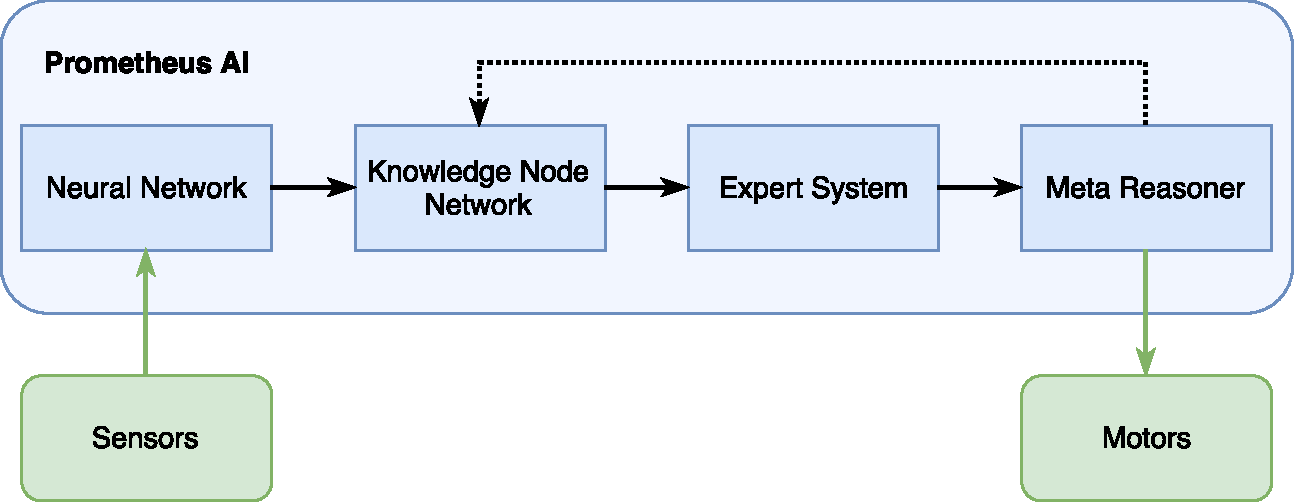
\includegraphics[width=\columnwidth]{figures/ai_model.pdf}
	\caption{Prometheus AI model.}
	\label{model}
\end{figure}

\section{Background}
\label{sec:background}
% In this section you should summarize the theory and background that you had to learn, and that you believe are necessary for the reader to understand the rest of the report.

\subsection{Neural Network}

The NN layer (also known as the Perceptron layer) consists of a network of neurons with a similar structure to neurons in the human brain. In the context of this project, it is the interface between the robots' sensors (camera and ultrasonic) and the rest of the AI system.

The NN layer gathers raw sensor data and will build an abstract view of the robot's surrounding environment. It will analyze the contents of the camera image and achieve two main goals:

\begin{enumerate}
	\item Classify objects observed in the image
	\item Localize objects in the image
\end{enumerate}

To achieve these goals, a convolutional neural network will be used. This will determine which regions of the image are important and classify objects in those regions. A 3D view of the world will also be generated. Using ultrasonic sensor readings and coordinate transformations from the world to the camera images, the observed objects can be localized in space.

Ultimately, the classification and localization of objects will produce abstract informational tags, which will be passed on to the KNN. These tags can therefore be measures of the position of an object, or other characteristics about an object.

% TODO: Put figure of robots with their sensors

\subsection{Knowledge Node Network}

The KNN layer represents memory in the human brain. It takes in the tags provided by the NN and outputs tags based on its knowledge of the environment. These output tags can be simple facts, such as ``I see a wall'', or can be recommendations for future actions such ``turn left''. These tags are passed on to the next layer, the Expert System (ES).

The KNN is based around the Knowledge Node, which is an abstract structure representing a memory and its connections to other memories. A simple model of a Knowledge Node can be seen in \ar{kn}.

\begin{figure}[!htb]
	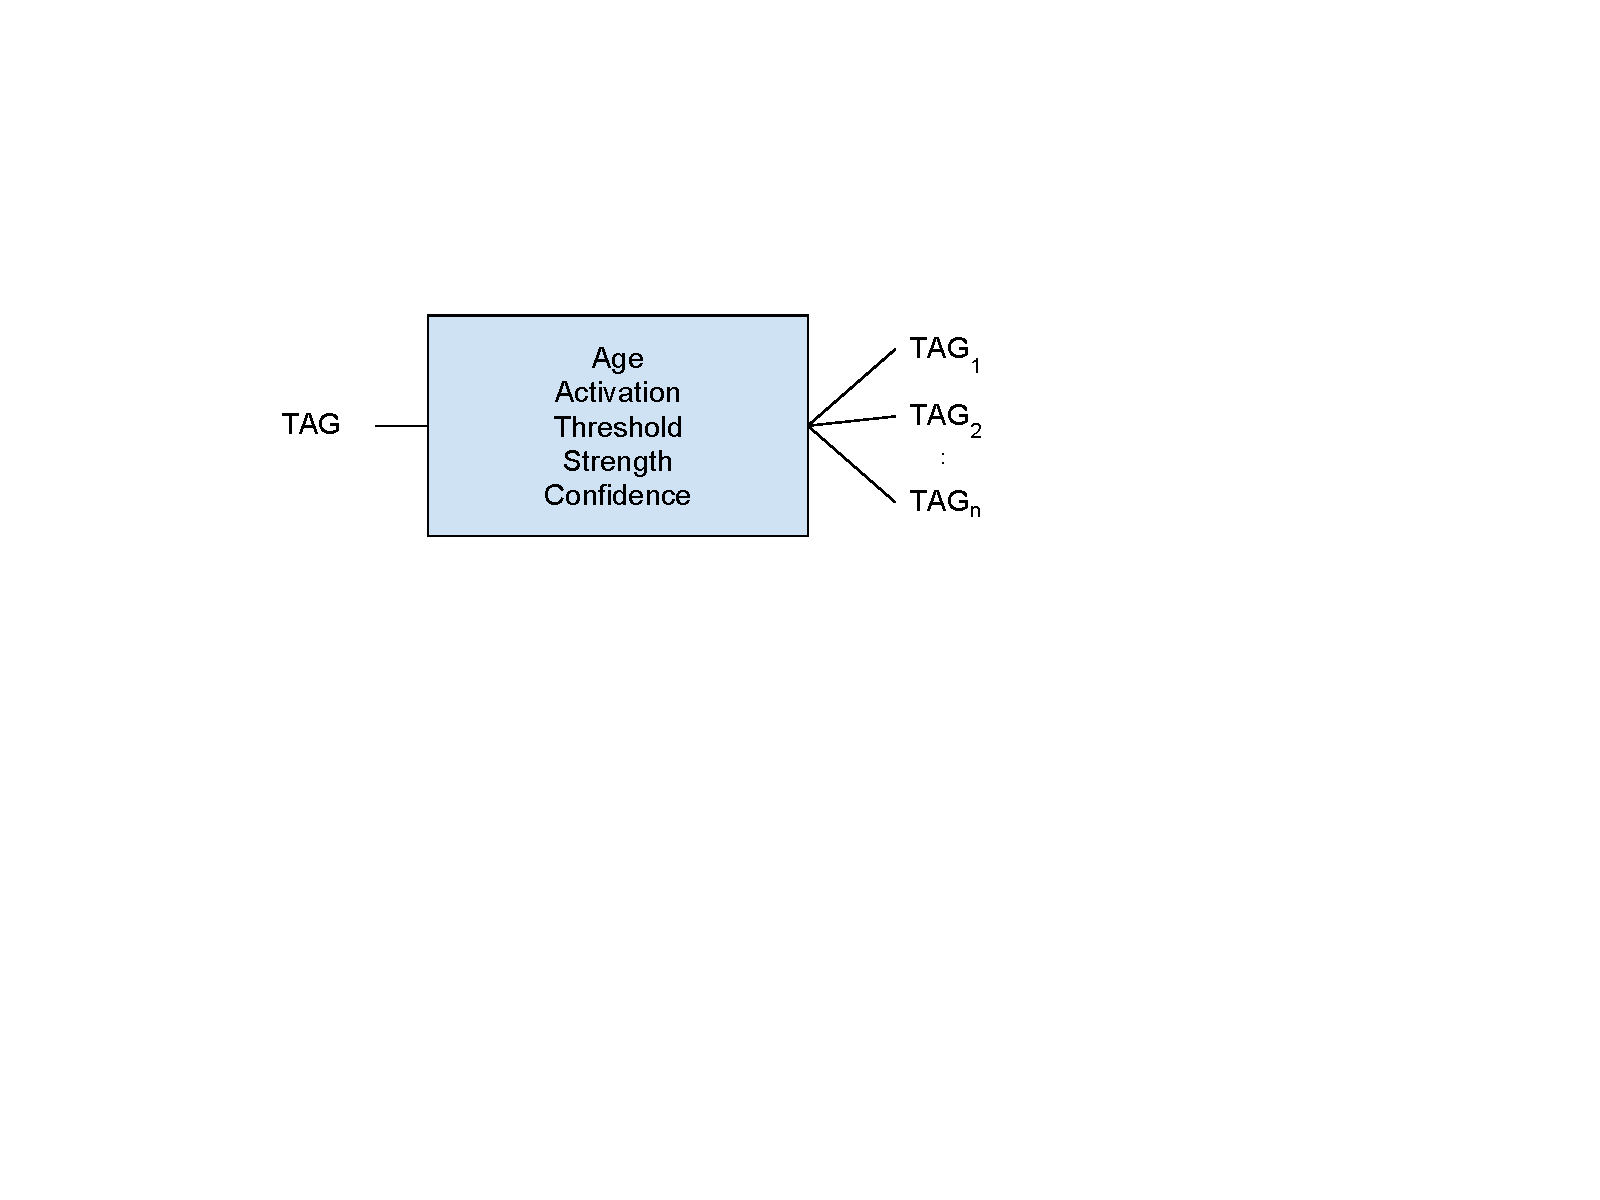
\includegraphics[width=\columnwidth]{figures/kn.pdf}
	\caption[High-level model of the Knowledge Node of the KNN.]
	{High-level model of the Knowledge Node of the KNN \cite{vybihal-knowledge}.}
	\label{kn}
\end{figure}

In its simplest form, the Knowledge Node can be excited by an activated input tag, which increments its activation parameter, which initially starts at 0. If the activation parameter is greater than the node's threshold, the Knowledge Node fires, causing the activation of the output tags. This description corresponds to forwards thinking with linear activation. The activation can also be with a sigmoid function, which is more representative of neurons in the brain.
% TODO: source ^^?
% TODO: talk more about relation to neurons in brain, and ways to leverage this

Other ways of thinking are also possible. Indeed, the KNN has three main ways of thinking: forwards, backwards, and lambda. The version of thinking to be done by the KNN is chosen by the META.

Forwards thinking is the simplest and was described earlier. It is depicted in \autoref{think_forwards}. Firing a Knowledge Node can cause forward activation of more Knowledge Nodes, hence the ``forwards'' naming.

\begin{figure}[!htb]
	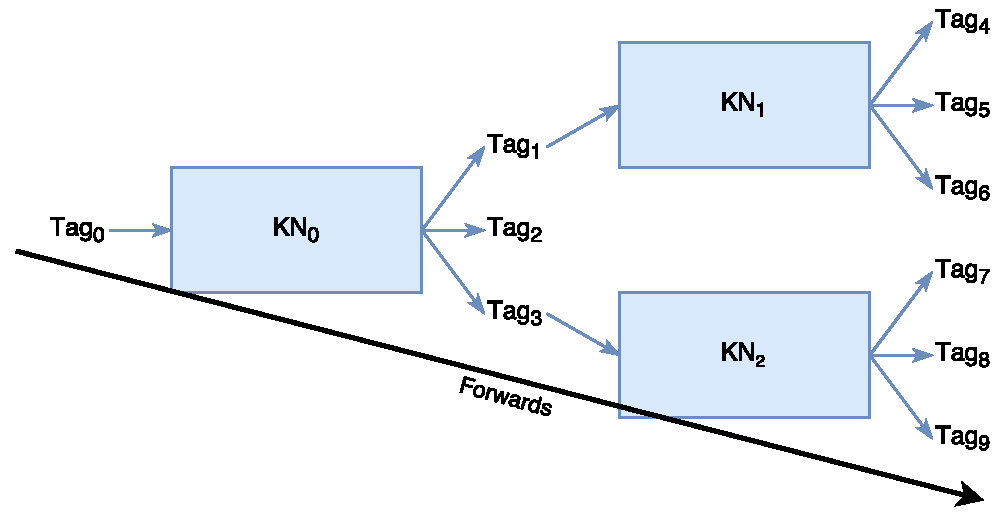
\includegraphics[width=\columnwidth]{figures/forwards_thinking.pdf}
	\caption{Thinking forwards in the KNN.}
	\label{think_forwards}
\end{figure}

Thinking backwards starts at the output tags of Knowledge Nodes, and works backwards, as can seen in \autoref{think_backwards}. In its simplest form, it checks output tags of Knowledge Nodes and, if all of them are active, the input tag must be active as well, so that Knowledge Node is activated.

This type of thinking can be a bit more difficult to implement than forwards thinking, since one must decide what percentage of active output tags of a Knowledge Node corresponds to an active input tag. For instance, should a Knowledge Node activate when all its output nodes are active (100\%), or when 75\% are active? This relates to the confidence with which the KNN believes the tag associated with that node to be true. As a concrete example, if you observe an object that has four wheels, seats, and a steering wheel, how confident are you that that object is a car? Realistically, humans with often classify what they observe with a certain uncertainty and this is what can be represented with this type of backwards thinking. The memories of this observation are then even more uncertain.
% TODO: source^^

This type of thinking occurs constantly in the background in humans \cite{vybihal-knowledge}, and this is something to keep in mind during implementation.
% TODO: source other than Vybihal here^^


\begin{figure}[!htb]
	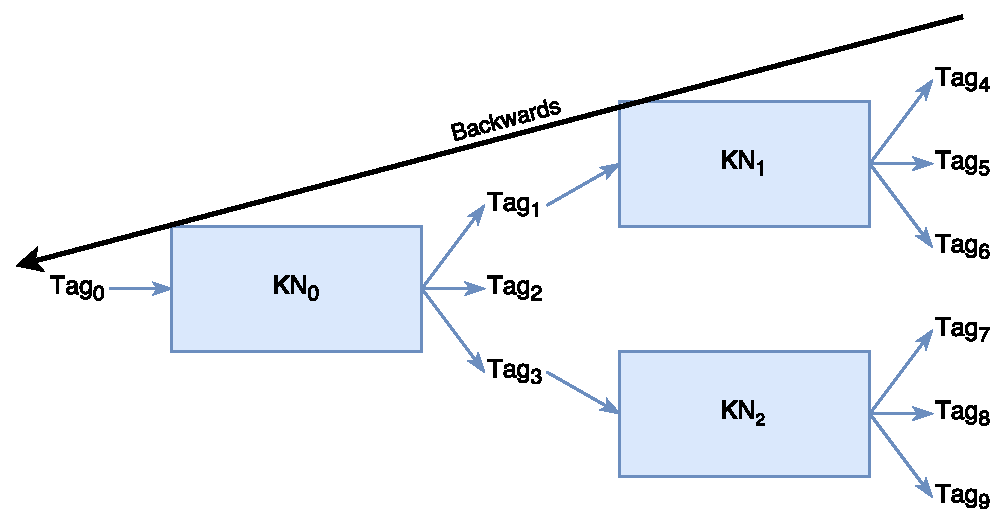
\includegraphics[width=\columnwidth]{figures/backwards_thinking.pdf}
	\caption{Thinking backwards in the KNN.}
	\label{think_backwards}
\end{figure}

Lambda thinking uses a combination of forwards and backwards, and can be seen in \autoref{think_lambda}. It is called ``lambda'' thinking because the shape of the thinking trajectory matches a Greek uppercase lambda ($\Lambda$). It first looks at output tags of Knowledge Nodes and propagates activation backwards, similar to backwards thinking. After a certain amount of nodes are fired, it will then start activating forwards, similar to thinking forwards. An interesting question is how far backwards should lambda thinking go before starting to cascade forwards? This relates to how general one wants to explore before searching for a more specific value.

This type of thinking occurs in humans when using analogical reasoning to solve problems \cite{vybihal-lambda}. In essence, when a person wants to find a solution to a problem, they will explore related problems, move their way ``backwards'' to concepts related to the desired problem, and think ``forwards'' to focus in on the desired problem.

\begin{figure}[!htb]
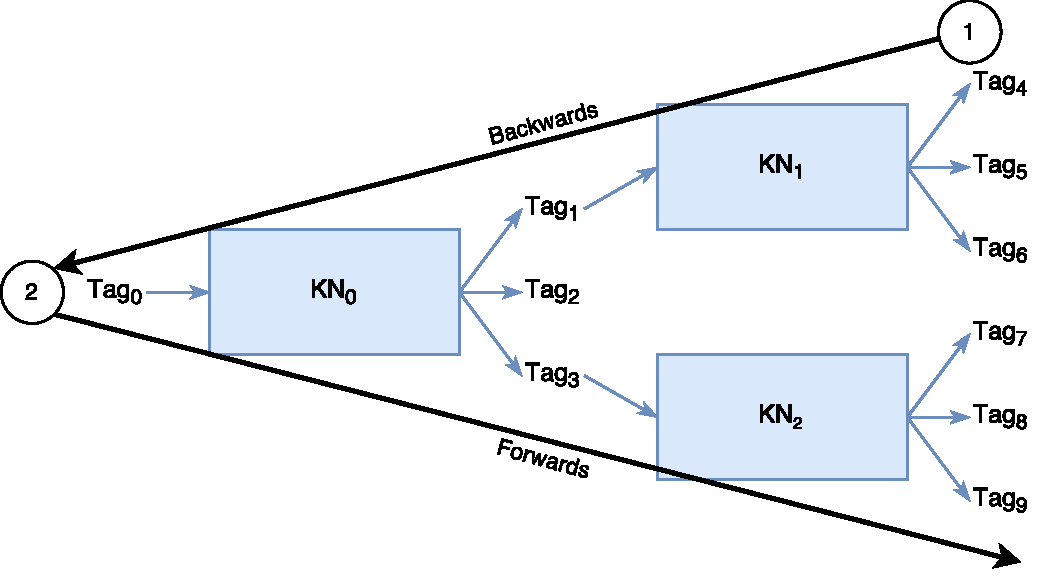
\includegraphics[width=\columnwidth]{figures/lambda_thinking.pdf}
\caption{Lambda thinking in the KNN.}
\label{think_lambda}
\end{figure}

All forms of thinking can continue until there are no more Knowledge Nodes to activate, which corresponds to natural quiescence. There can also be a fixed number of cycles through the list of active tags. This fixed cycle number represents how much effort is being put into thinking. Indeed, in animals, most thinking is never done at 100\% effort, and it would be interesting to model this.

\subsection{Expert System}

The ES layer is a basic logic reasoner. It is not aware of its current reality, or any context. It takes in the tags provided by the KNN and interprets them as either facts, recommendations or rules.

Facts are simple calculus predicates showing that something is true. For example, the fact $(A)$ represents that $A$ itself is true or active, $(A = 1)$ means that $A$ is equal to 1, $(A > 1)$ represents that $A$ is greater than 1, etc. As a more concrete example, a fact can represent a certain measurement, like $(distance = 5)$ representing the robot's distance from a wall as measured by one of its sensors.

Recommendations represent suggestions for actions to be taken by a robot. For example, $(\#turn\_left)$ is a recommendation for a robot to turn left, if it sees a wall directly in front of it and must avoid it, for example. These are recommendations and not commands because the META can decide whether or not to actually take that action.

Rules are a many-to-many structure with facts or recommendations as inputs and outputs. When all the input tags become active, the output tags become active and the rule itself is also said to be active. In this way, a rule can represent a logical AND of all its input tags.

The runtime of the ES consists of the following general steps \cite{vybihal-expert}:

\begin{enumerate}
	\item Reset
	\item Add facts and rules
	\item Think
	\item Send recommendations to META
\end{enumerate}

The most important part of the previous process is the thinking stage, which consists of first iterating through all the rules in the ES and checking if they are active by inspecting the lists of facts and recommendations. Rules may then become active and cause cascading activation of more rules. This can continue until there are no more rules to activate, which corresponds to natural quiescence. There can also be a fixed threshold to the number of possible cycles through the lists of facts and recommendations. In this sense, this limit represents the effort put into thinking, similarly to the KNN.

These recommendations are passed on to the final layer, the Meta Reasoner (META).

\subsection{Meta Reasoner}

The META layer represents high-level reasoning in human brains. It is aware of its environment and context, and makes decisions based on what it believes to be right. It is paranoid, and constantly checks whether the tags reported by the rest of the AI system make sense based on its expected view of the world. If it decides to make a decision, it sends a command to the actuators of the robots to decide how to move. If it is not happy with the recommendation(s) from the ES, it may initiate another think cycle in the KNN to generate new recommendations(s).

\subsection{Summary}

With this full description of the Prometheus AI model, the system with labeled input and output can be seen in \autoref{model_labeled}.

\begin{figure*}[!htb]
	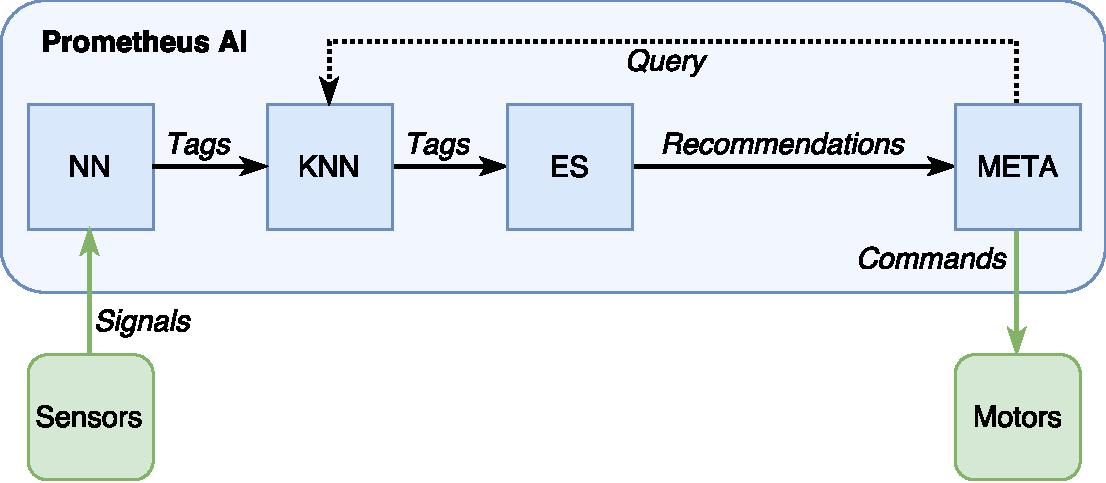
\includegraphics[width=\textwidth]{figures/ai_model_labeled.pdf}
	\caption{Prometheus AI model with labeled input and output.}
	\label{model_labeled}
\end{figure*}

\section{Problem}
% In this section you should describe the problem or system you are addressing in detail. Describe the project requirements and constraints.

The assigned task was to construct two out of the four layers listed in \autoref{sec:background}: the Expert System (ES), and the Knowledge Node Network (KNN). The other two layers are to be completed by another Honours Thesis student.

As a deliverable for the end of this first semester, it was required to complete a prototype of these two layers, with basic versions of the functionality described in \autoref{sec:background}. This was to be done entirely in Java.

\section{Design Criteria}
% In this section you must describe any design work that was already completed. Discuss any design decisions that have been made, and describe the process that was followed to make these decisions. Also discuss any results that have already been obtained this semester.

\subsection{Efficiency}

A very important consideration when designing the system is speed. Since the robots may have to react very quickly to stimulus in the environment, the reasoning in the AI must be as fast as possible. This is especially true in the hazardous environments for which this system could be useful for, as specified in \autoref{sec:intro}. An example of a design choice that was made to improve speed is the use of Java Sets for most of the collections in the ES and KNN layers. The original specifications mentioned using ArrayLists, but, since there is no specific iteration order necessary for most operations in the ES and KNN, these collections were changed to Sets.

When designing every algorithm in the system, the first criterion in mind is speed. Indeed, for the \code{think()} methods of the ES and KNN, it was important to think about the right way to leverage all the available data structures to maximize speed.

\subsection{Object Oriented Design}

Another important choice is to leverage object-oriented design as much as possible. Object-oriented programming (OOP) allows extensive planning before even beginning to write code, which can identify any flaws in the initial design. It also allows the code to be very clean and reusable. Since Java is the programming language chosen for the project, OOP is also the natural way to proceed. To follow OOP, the ES and KNN will be designed around Java classes and the methods associated with those classes. OOP principles such as polymorphism and encapsulation will be followed closely.

\subsubsection{Abstraction}

One important design aspect is that the system should be as abstract as possible, while still performing its desired task. For instance, the system should be general enough to perform under simulations, as well as in real-life environments. It should also ideally be able to perform in vastly different environments, with different tasks.

One example of making use of abstraction is the choice to create a \code{PrometheusLayer} interface for both the ES and KNN, since they share some functionality, like the ability to think.

\subsubsection{Encapsulation}

Each layer of the system has unique, localized functionality that does not need to be visible from the rest of the system. For instance, the intricacies of the \code{think()} method in the ES and KNN layers do not need to be known to the rest of the system.

\subsubsection{Polymorphism}

Many methods in the system can have different functionality depending on context. For instance, the \code{think()} method in the KNN and ES layers can take an optional number of think cycles to specify a threshold for quiescence.

\subsubsection{Inheritance}

Careful thought was put into how objects may inherit functionality from each other. This can most clearly be seen with the implementation of the tags, which will be described in \autoref{sec:implementation}.

\section{Implementation}
\label{sec:implementation}

The details of how the KNN and ES were implemented in Java will now be discussed.

\subsection{Tags}

The entire system revolves around tags passed from layer to layer. For this reason, a lot of thought was put into the proper design of these tags. To leverage OOP principles and readability, it was decided to implement these tags with a \code{Tag} class in Java, with \code{Fact}, \code{Rule} and \code{Recommendation} subclasses.

The tags described in \autoref{sec:background} need to be as general as possible. A natural choice for this structure would be a Java \code{String}, which would be relatively simple to pass around the system. However, these tags represent various concepts; each tag can either be a fact, a recommendation, or a rule. If implemented as \code{String}s, the tags would have to be encoded on creation to represent each concept and decoded on use to retrieve the important information. This seems like a bad use of the OOP principles of Java. For this reason, the tags are instead implemented using a \code{Tag} Java class, with \code{Recommendation}, \code{Fact}, and \code{Rule} subclasses. This should also make manipulating the Tags faster, while incurring a slight memory overhead. To store these Tags in a database, they can be converted to JSON format. On read from the database, they can be easily decoded.

The \code{Tag} class itself was made abstract. This means that an object may not be directly instantiated as a \code{Tag}, but must be instantiated as one of its subclasses. This makes sense, since a tag \emph{must} be one of the three types: rule, recommendation or fact.

All of these classes were placed inside the \code{tags} package. A UML diagram of the \code{tags} package can be seen in \autoref{uml_tags} of the Appendix.

\subsection{Knowledge Node Network}

All code relating directly to the KNN was placed in the \code{knn} package of the project. A UML diagram of the \code{knn} package can be seen in \autoref{uml_knn} of the Appendix.

The KNN layer is based around the \code{KnowledgeNodeNetwork} Java class. This class has the following fields:

\begin{labeling}{\code{activeTags}}
	\item[\code{mapKN}] \code{Map} of input \code{Tags} to associated \code{KnowledgeNodes}
	\item[\code{activeTags}] \code{Set} of active \code{Tags}, corresponding to input \code{Tags} of fired \code{KnowledgeNodes}
\end{labeling}

The \code{KnowledgeNode} class implements the functionality of a Knowledge Node, which has the following important fields implemented functionality described in \autoref{sec:background}:

\begin{labeling}{\code{outputTags}}
	\item[\code{inputTag}] input \code{Tag}.
	\item[\code{outputTags}] \code{Array} of output \code{Tags}.
	\item[\code{activation}] \code{int} starting at 0, incrementing when the \code{KnowledgeNode} is excited.
	\item[\code{threshold}] \code{int} threshold such that \code{activation $\geq$ threshold} causes firing of the \code{KnowledgeNode}.
	\item[\code{strength}] \code{int} that biases the activation of a \code{KnowledgeNode}, causing early firing. Simple implementation: if \code{activation * strength $\geq$ threshold} then fire the KN.
	\item[\code{confidence}] \code{int} representing the belief that \code{inputTag} is true (0 to 100\%).
	\item[\code{age}] \code{int} representing the age of the \code{KnowledgeNode}.
\end{labeling}

The most important method in the \code{KnowledgeNodeNetwork} is \code{think()}, which chooses either \code{thinkForwards()}, \code{thinkBackwards()}, or \code{thinkLambda()}. These methods implement the functionality described in \ar{sec:background} and return the \code{Tags} activated as a result of thinking.

Without a parameter, the \code{think()} method runs to natural quiescence. There is also an overloaded version of \code{think()} that takes an \code{int} \code{numberOfCycles} as a parameter. This parameter represents the thinking effort described earlier. Similarly, \code{thinkForwards()}, \code{thinkBackwards()}, and \code{thinkLambda()} all have overloaded versions with \code{numberOfCycles} as a parameter.

Currently, only the \code{thinkForwards()} method is fully completed. The version of the method that runs until quiescence can be seen in \autoref{lst:thinkForwards}.

\lstinputlisting[
firstline=162,
lastline=170,
caption=Thinking forwards until quiescence in the KNN.,
label=lst:thinkForwards
]{
	\knnpath
}

The version of \code{thinkForwards()} with a fixed number of thinking cycles can be seen in \autoref{lst:thinkForwardsThreshold}.

\lstinputlisting[
firstline=178,
lastline=188,
caption=Thinking forwards for a fixed number of cycles in the KNN.,
label=lst:thinkForwardsThreshold
]{
	\knnpath
}

One can see that the \code{thinkForwards()} methods repeatedly call \code{forwardThinkCycle()}, which can be seen in \autoref{lst:forwardThinkCycle}. This method is where \code{Tags} can become active, being added into the \code{activeTags} \code{Set}.

\lstinputlisting[
firstline=195,
lastline=203,
caption=Single cycle of thinking forwards in the KNN.,
label=lst:forwardThinkCycle
]{
	\knnpath
}

One can see that the \code{forwardThinkCycle()} calls an \code{excite()} method to excite a \code{KnowledgeNode}. This method returns the \code{Tags} activated as a result of excitation. The code can be seen in \autoref{lst:excite}.

\lstinputlisting[
firstline=212,
lastline=219,
caption=Method to excite a Knowledge Node.,
label=lst:excite
]{
	\knnpath
}

This method, in turn, may call a \code{fire()} method to fire the \code{KnowledgeNode} and activate its output tags. It returns all the \code{Tags} to be activated as a result of firing that \code{KnowledgeNode}. The code can be seen in \autoref{lst:fire}.

\lstinputlisting[
firstline=227,
lastline=235,
caption={Method to fire a Knowledge Node, activating its output tags.},
label=lst:fire
]{
	\knnpath
}

\subsection{Expert System}

All code relating directly to the ES was placed in the \code{es} package of the project. A UML diagram of the \code{es} package can be seen in \autoref{uml_es} of the Appendix.

The ES layer is based around the \code{ExpertSystem} Java class. This class has the following fields:

\begin{labeling}{\code{recommendations}}
	\item[\code{readyRules}] \code{Set} of \code{Rules} that have not been activated yet.
	\item[\code{activeRules}] \code{Set} of active \code{Rules}.
	\item[\code{facts}] \code{Set} of active \code{Facts}.
	\item[\code{recommendations}] \code{Set} of active \code{Recommendations}.
\end{labeling}

The most important method in the \code{ExpertSystem} is \code{think()}, which chooses either \code{thinkForwards()}, \code{thinkBackwards()}, or \code{thinkLambda()}. These methods implement the functionality described in \ar{sec:background}.

Without a parameter, the \code{think()} method runs to natural quiescence. This can be seen in \autoref{lst:think}.

\lstinputlisting[
firstline=153,
lastline=166,
caption=Thinking until quiescence in the ES.,
label=lst:think
]{
	\espath
}

There is also an overloaded version of \code{think()} that functions similarly to that of the \code{KnowledgeNodeNetwork}. This can be seen in \autoref{lst:thinkThreshold}. Both variants of \code{think()} return the \code{Set} of \code{Recommendations} that become active as a result of thinking, which is passed on to the META.

\lstinputlisting[
firstline=178,
lastline=192,
caption=Thinking with a fixed number of cycles in the ES.,
label=lst:thinkThreshold
]{
	\espath
}

Both versions of \code{think()} call a method named \code{thinkCycle()} representing a single cycle of thinking. The code for this method can be seen in \autoref{lst:thinkCycle}. This is the method where \code{Rules} and \code{Recommendations} can become active within the ES.

\lstinputlisting[
firstline=202,
lastline=228,
caption=A single cycle of thinking in the ES.,
label=lst:thinkCycle
]{
	\espath
}

\subsection{Testing}

All tests on the system were conducted using the TestNG framework in Java, which provides a simple and intuitive way to create assertions in tests. These tests were placed in the \code{test} package of the project. A UML diagram of the \code{test} package can be seen in \autoref{uml_test} of the Appendix.

\subsubsection{Unit Tests}

Unit tests were generated for the KNN and ES to test every single method on its own.

\subsubsection{Integration Tests}

Integration tests were made to test the combined functionality of the KNN and ES.

The test setup for the \code{testKNN()} method can be seen in \autoref{testKNN}. Every node has a \code{threshold} value of 1 to simplify the activation. The system starts out with $A$ as the only active \code{Tag}, and \code{testKNN()} with \code{think()} until quiescence. It is therefore expect all the \code{Tags} shown in \autoref{testKNN} to become active at the end. The initial and final states are both asserted with TestNG in \code{testKNN()}, with positive results.

\begin{figure*}[!htb]
	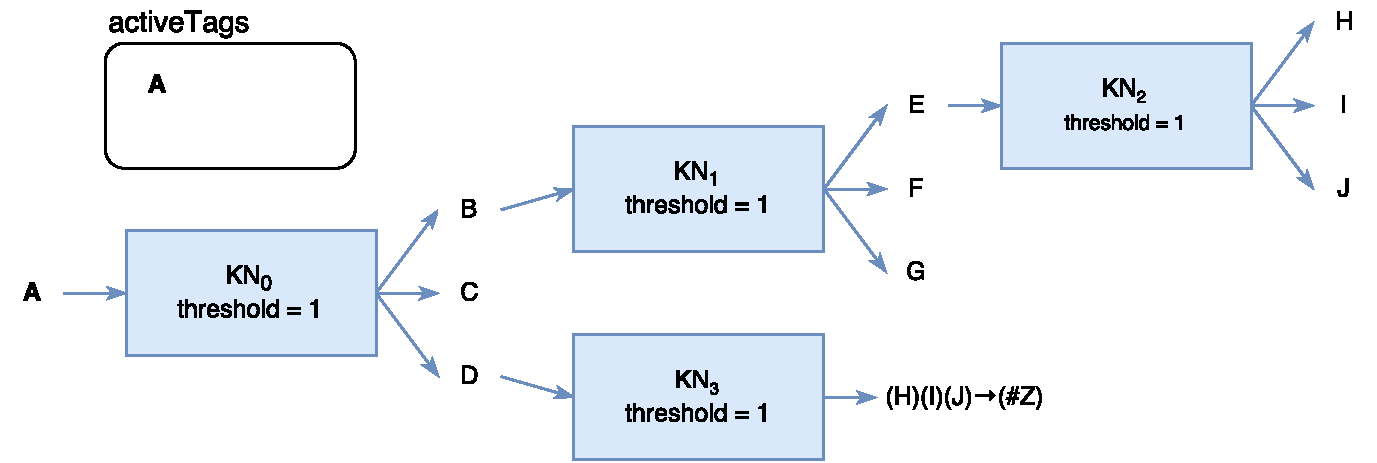
\includegraphics[width=\textwidth]{figures/testKNN.pdf}
	\caption[Setup for the \code{testKNN()} method.]
	{Initial setup for the \code{testKNN()} method.}
	\label{testKNN}
\end{figure*}

The test setup for the \code{testES()} method can be seen in \autoref{testES}. The columns from left to right correspond to the elements in the \code{readyRules}, the \code{activeRules}, the \code{facts}, and the \code{recommendations} respectively. The first row corresponds to the initial setup of the ES, and the last row corresponds to the expended final state. Both the initial and final states are asserted with TestNG in \code{testES()}, with positive results.

\begin{table*}[!htb]
	\large
	\centering
	\begin{tabular}{c | c | c | c} 
		\textbf{Ready Rules} & \textbf{Active Rules} & \specialcell{\textbf{Active} \\ \textbf{Facts}} & \specialcell{\textbf{Active} \\ \textbf{Recommendations}}  \\ \hline
		\specialcell{$(A)(B)\rightarrow(D)$ \\ $(D)(B)\rightarrow(E)$ \\ $(D)(E)\rightarrow(F)$\\ $(G)(A)\rightarrow(H)$ \\ $(\#X)(\#Y)\rightarrow(\#Z)$} &  & $(A),(B)$ & $(\#X),(\#Y)$ \\ \hline
		$\vdots$ & $\vdots$ & $\vdots$ & $\vdots$ \\ \hline
		$(G)(A)\rightarrow(H)$ & \specialcell{$(A)(B)\rightarrow(D)$ \\ $(D)(B)\rightarrow(E)$ \\ $(D)(E)\rightarrow(F)$ \\ $(\#X)(\#Y)\rightarrow(\#Z)$} & \specialcell{$(A),(B),$ \\ $(D),(E)$ \\ $(F)$} & $(\#X),(\#Y),(\#Z)$		
	\end{tabular}
	\caption[Test setup for \code{testES()}.]
	{Test setup for \code{testES()}. Middle activation steps omitted.}
	\label{testES}
\end{table*}

The \code{testKNNandES()} method has the same setup as \code{testKNN()} in \autoref{testKNN}, except the output active Tags from the KNN are passed on to the ES. The resulting setup and activation in the ES can be seen in \autoref{testKNNandES}.

\begin{table*}[!htb]
	\large
	\centering
	\begin{tabular}{c | c | c | c | c} 
		\textbf{Cycle} & \textbf{Ready Rules} & \textbf{Active Rules} & \specialcell{\textbf{Active} \\ \textbf{Facts}} & \specialcell{\textbf{Active} \\ \textbf{Recommendations}}  \\ \hline
		1
		&$(H)(I)(J)\rightarrow(\#Z)$
		& 
		& \specialcell{$(B),(C),(D)$ \\ $(E),(F),(G)$ \\ $(H),(I),(J)$}
		& \\ \hline
		
		2
		&
		& $(H)(I)(J)\rightarrow(\#Z)$
		& \specialcell{$(B),(C),(D)$ \\ $(E),(F),(G)$ \\ $(H),(I),(J)$}
		& $(\#Z)$
	\end{tabular}
	\caption{Test setup and activation for the ES portion of \code{testKNNandES()}.}
	\label{testKNNandES}
\end{table*}

\subsection{Documentation}

Proper documentation of the source code is very important. This is to ensure that anyone wanting to work with the code which was designed has an easy time doing so. Also, for anyone wanting to understand how the system works, documentation is essential. This documentation was achieved through Javadoc and UML diagrams.

\subsubsection{Javadoc}

Extensive Javadoc was generated for the entire code base. This can be found here: \url{http://cs.mcgill.ca/~sstapp/prometheus/index.html}. The functionality of every single class and method was described in detail.

\subsubsection{UML}

UML diagrams of every package in the code base were created.

\section{Plan for Next Semester}
% In this section you should describe a plan for next semester. What tasks remain to be done, and what is the timeline for accomplishing these tasks? Furthermore you can describe how you plan to test your design in order to make sure it meets the desired specifications. Also outline the design decisions that are required in order to make sure that the final product can be tested.
% TODO: Maybe include schedule

The plan for next semester is to finalize the two layers that were started this semester, and to test them on the robots available in Prof. Vybihal's lab.

\subsection{Finalization}

\subsubsection{Knowledge Node Network}

Many complex features of the KNN layer are still to be implemented, such as backwards and lambda thinking, confidence, and aging.

Backwards thinking can be implemented using a background thread in Java, constantly running in the background at some rate.

Some thought still needs to be put into the specifics on implementation of lambda thinking. Most importantly, the use cases of lambda thinking will have to be well understood and described.

Confidence values will probably be associated with every individual \code{Tag}, as well as in an absolute sense in the KNN. Activation through the layers of the KNN can theoretically then reduce the absolute confidence that the output \code{Tags} are true, since at every step the confidence should be multiplied with the previous value.

The intuitive implementation of aging is to constantly increment some age value associated with every Knowledge Node, and discard nodes whose age is greater than some threshold. The age would be reset when the node is excited. This would however be unnecessarily computationally intensive, requiring some kind of constant updating of every single node. A more efficient way of doing it would be to save a timestamp for every Knowledge Node when it is excited, and if the KNN attempts to excite a Knowledge Node whose previous timestamp value is too far into the past, that node is instead deleted.

Activation of Knowledge Nodes with sigmoid functions can also be looked into. This can be easily implemented using a cache of known sigmoid values.

Also, more thought will have to be put into the design of the KNN to allow cyclic graphs, representing recursive memories in the human brain.

\subsubsection{Expert System}

Some features of the ES layer are still to be implemented, such as more complex Fact checking.

\subsection{Integration}

One very important task left to be done is to integrate the two layers described in this report (ES and KNN) with the other layers developed separately (NN and META). Ideally, the layers should be able to work together, but there will surely be some conflicts at the interface of the layers. These will have to be resolved when the time comes.

\subsection{Testing}

\subsubsection{Simulation}

Once all the layers are functioning together, they can be tested. The first and easiest way to test would be in a simulated environment. One simulator that may be used is Simbad, which is a Java 3D robot simulator \cite{simbad}. This can allow for some early debugging and fixes.

\subsubsection{Physical}

One the simulation testing is completed and working properly, the system can be tested in the lab. Prof. Vybihal's lab has multiple robots with ultrasonic sensors, and these will be the test subjects of this phase.

\section{Impact on Society and the Environment}
% In one or two pages, discuss the environmental and/or social impact of your project. Your analysis should include your work at McGill as part of this project, however, the main focus should be on the product/system you are designing (e.g., the cost/benefit/risk of manufacturing it, the cost/benefit/risk for consumers using it) or the problem your thesis is addressing (e.g., how will solving the problem influence/affect/benefit society and the environment). Particular emphasis should be given to:


\subsection{Use of Non-renewable Resources}
% Consider all stages of the product from design, manufacturing, distribution, use by consumers, and disposal/recycling.

As a purely software-oriented project, there are no physical materials needed to construct this system.

\subsection{Environmental Benefits}
% Benefits to the environment, comparisons with more polluting technologies etc.

The system could be used as a tool to control robots in dangerous environments such as nuclear plants after a radioactive disaster. Indeed, the system could coordinate robots to help contain the damage faster than humans could, thus limiting the risk on the environment.

\subsection{Safety and Risk}
% To you undertaking the project, as well as to any potential users of the solution once it is finished.

It is critical that, once this system is completed, it is used in an ethical way, and for the right purposes.

One example of use that may cause ethical concern is in a military setting, where an AI system like the one described here could be used in a battlefield in place of soldiers.

In the very long term, there are concerns with the possibility that an AI system might achieve intelligence and awareness close to a human. If such an AI were to obtain ``consciousness'' in its own way, should that entity be entitled to its own rights, like humans do?

\subsection{Benefits to Society}
% Quality of life, economic benefits, etc.

Going back to the example use case in a radioactive disaster, the system could be used to send robots in an area that would otherwise be very dangerous for humans. This would therefore help prevent the unnecessary loss of life in cleaning up these leaks.

\section{Conclusion}
% Use this section to summarize what was accomplished in this semester, provide a summary of the next steps and share any insight you have learned.

This semester, prototypes of the Expert System (ES) and Knowledge Node Network (KNN) layers of the AI model were completed in Java. These prototypes were tested individually and together, with positive results.

The main goal for next semester is to finalize the entire system, implementing more complex features that were omitted for this prototype stage.

\clearpage
\onecolumn
\appendix

\section{UML Diagrams}
\label{sec:uml}

\begin{figure}[!htb]
	\centering
	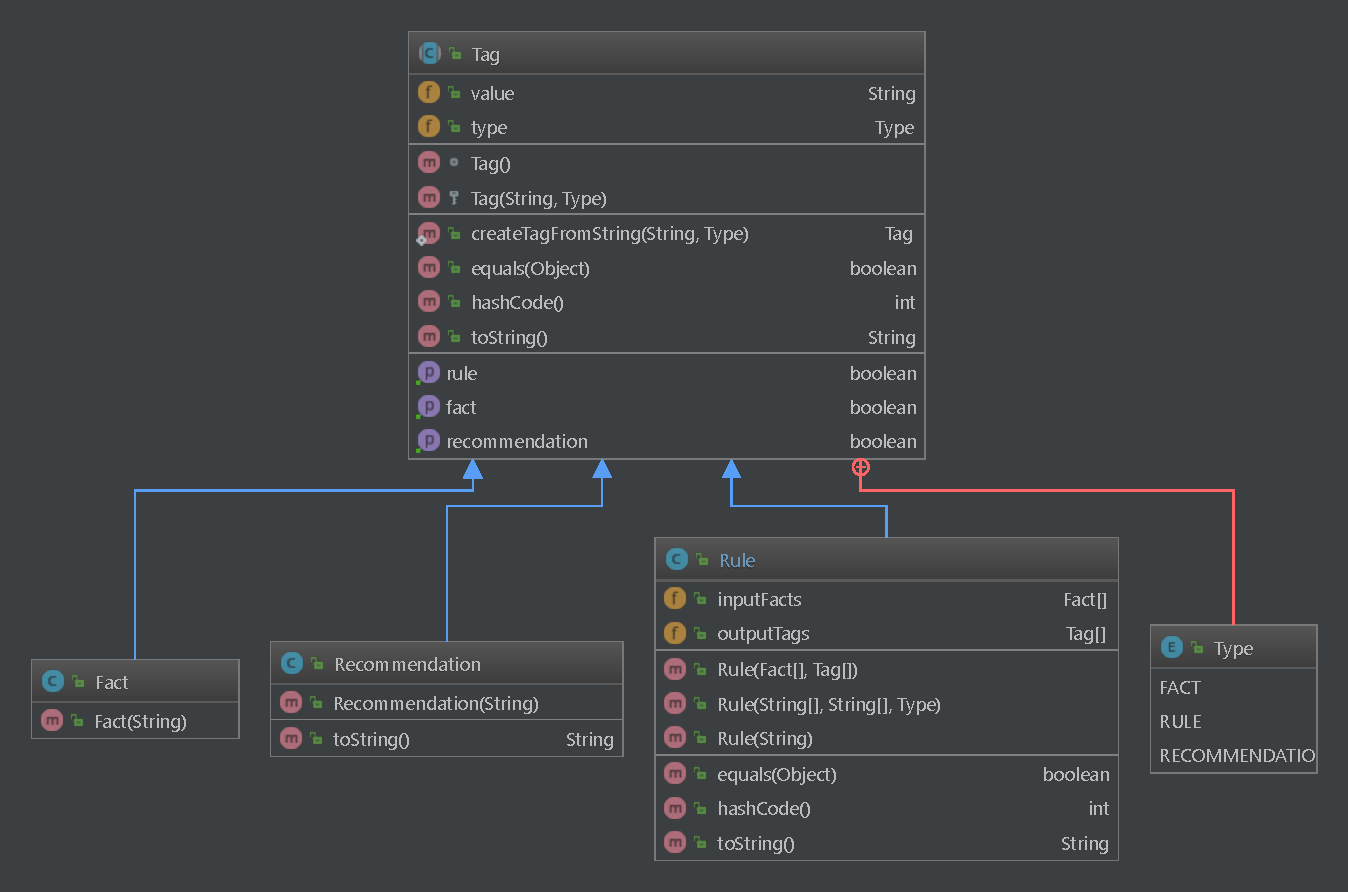
\includegraphics[width=\columnwidth]{figures/uml_tags.pdf}
	\caption{UML diagram of the \code{tags} package.}
	\label{uml_tags}
\end{figure}

\begin{figure}[!htb]
	\centering
	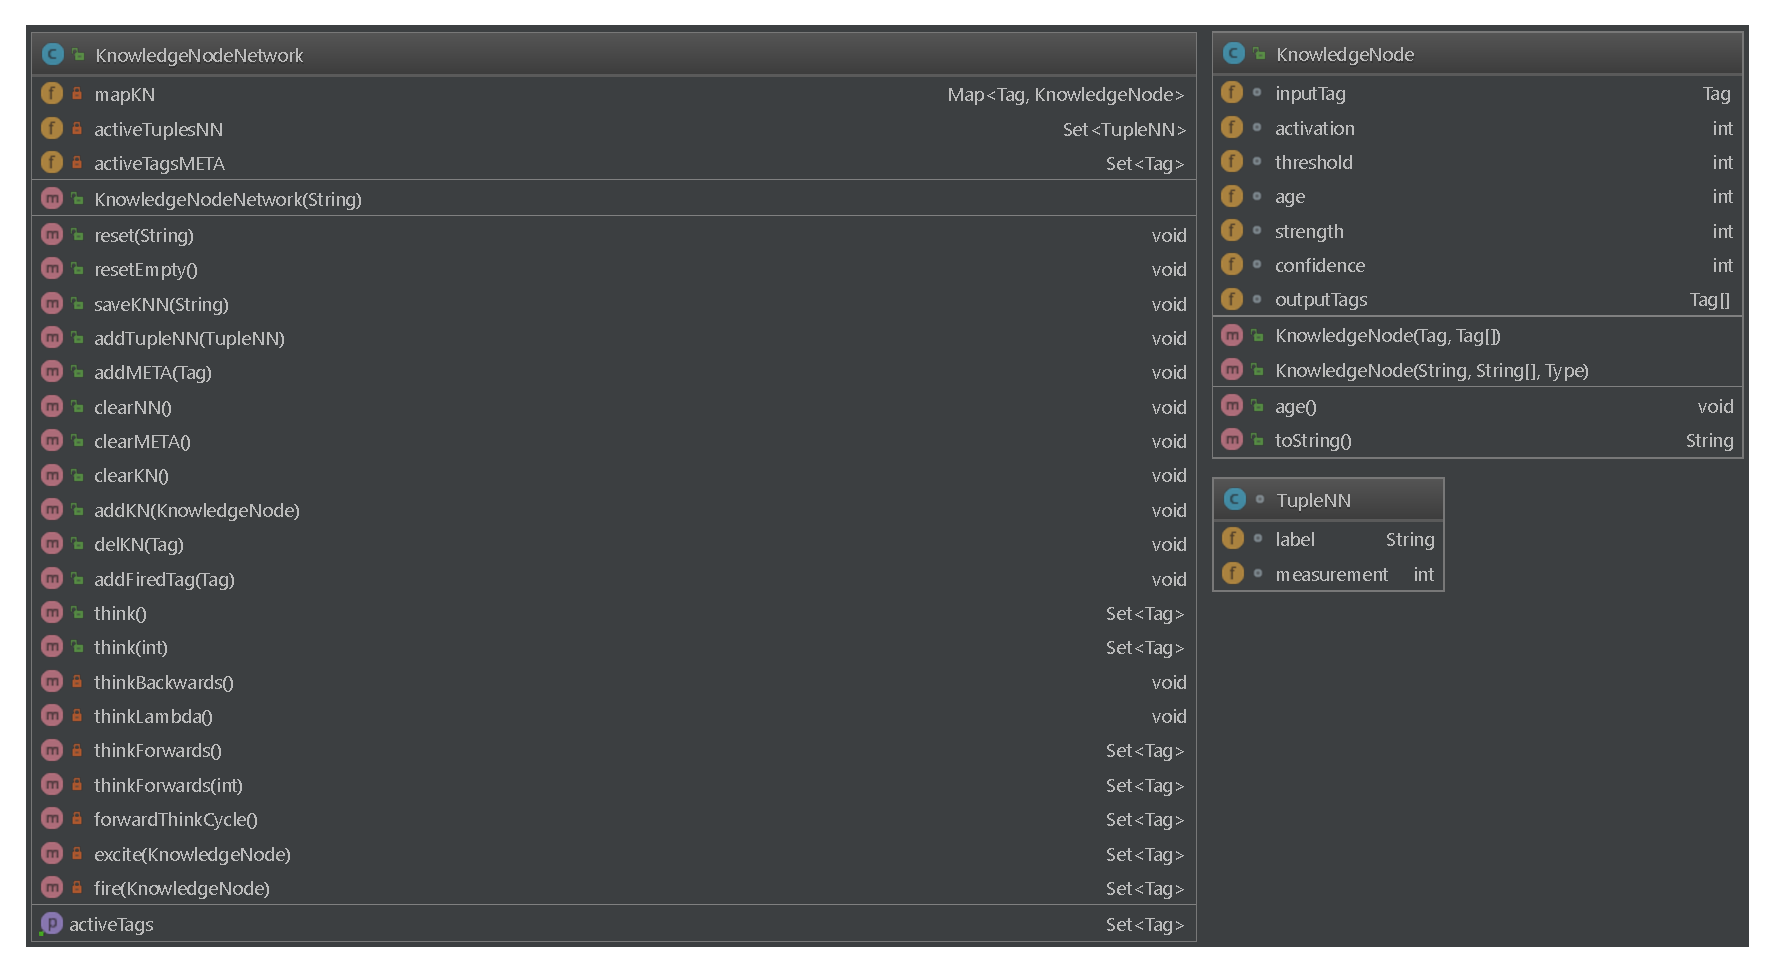
\includegraphics[width=\columnwidth]{figures/uml_knn.pdf}
	\caption{UML diagram of the \code{knn} package.}
	\label{uml_knn}
\end{figure}

\begin{figure}[!htb]
	\centering
	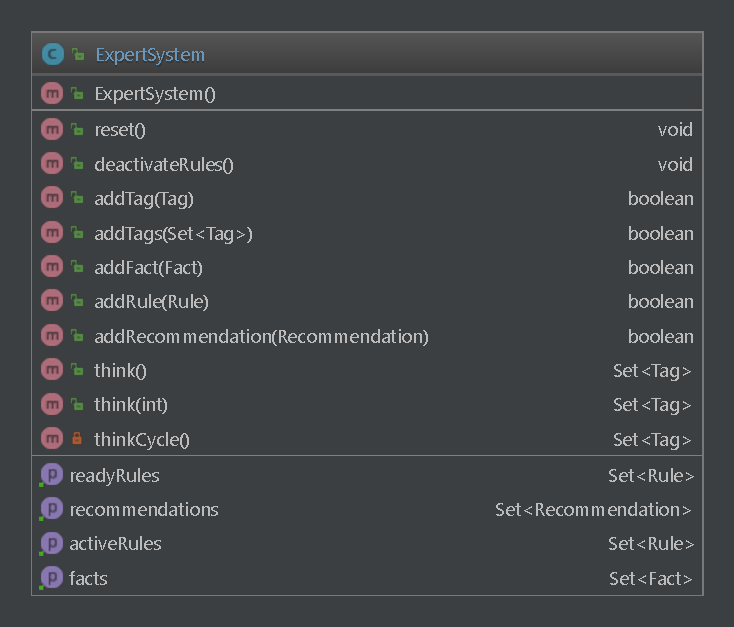
\includegraphics[width=0.5\columnwidth]{figures/uml_es.pdf}
	\caption{UML diagram of the \code{es} package.}
	\label{uml_es}
\end{figure}

\begin{figure}[!htb]
	\centering
	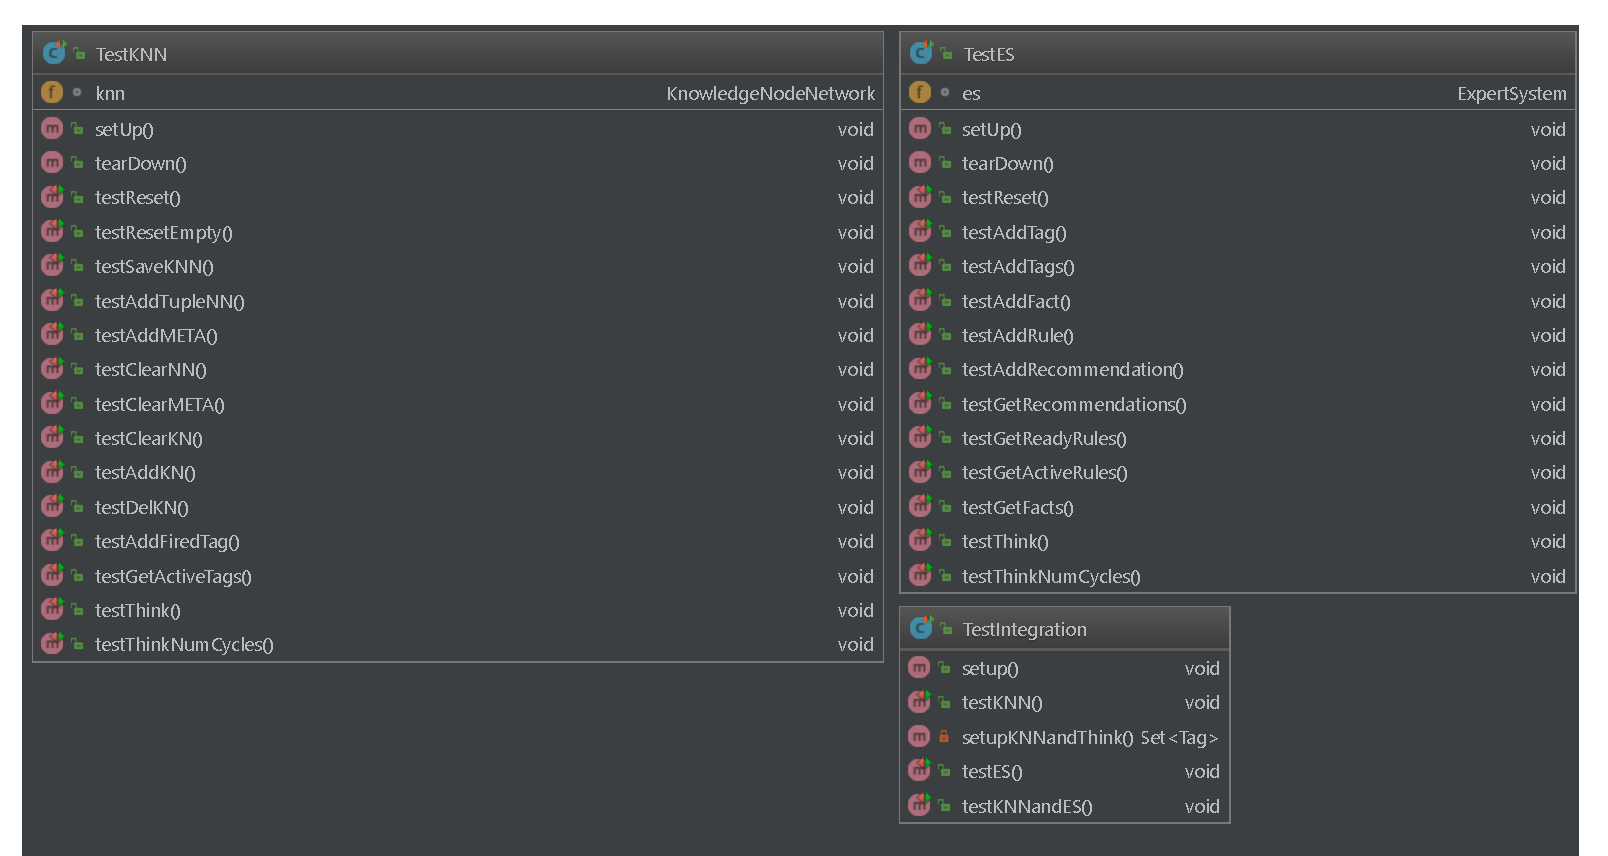
\includegraphics[width=\columnwidth]{figures/uml_test.pdf}
	\caption{UML diagram of the \code{test} package.}
	\label{uml_test}
\end{figure}

\clearpage

\bibliography{readings}{}
\bibliographystyle{IEEEtran}

\end{document}